\section{Implementation}
This section provides a comprehensive overview of the system's implementation. It includes the user interface illustrating each component and feature implemented in our email marketing tool during the first sprint. The user interface was designed to be simple and user-friendly. The goal was to make the tool easy to use even for users without much technical expertise

\subsection{Authentication Interface}

For the authentication interface, I decided to use JSON Web Tokens (JWT) for authentication. This decision was made due to JWT’s ability to securely transmit information between parties as a JSON object. This information can be verified and trusted because it is digitally signed.

\begin{figure}[ht]
	\centering
	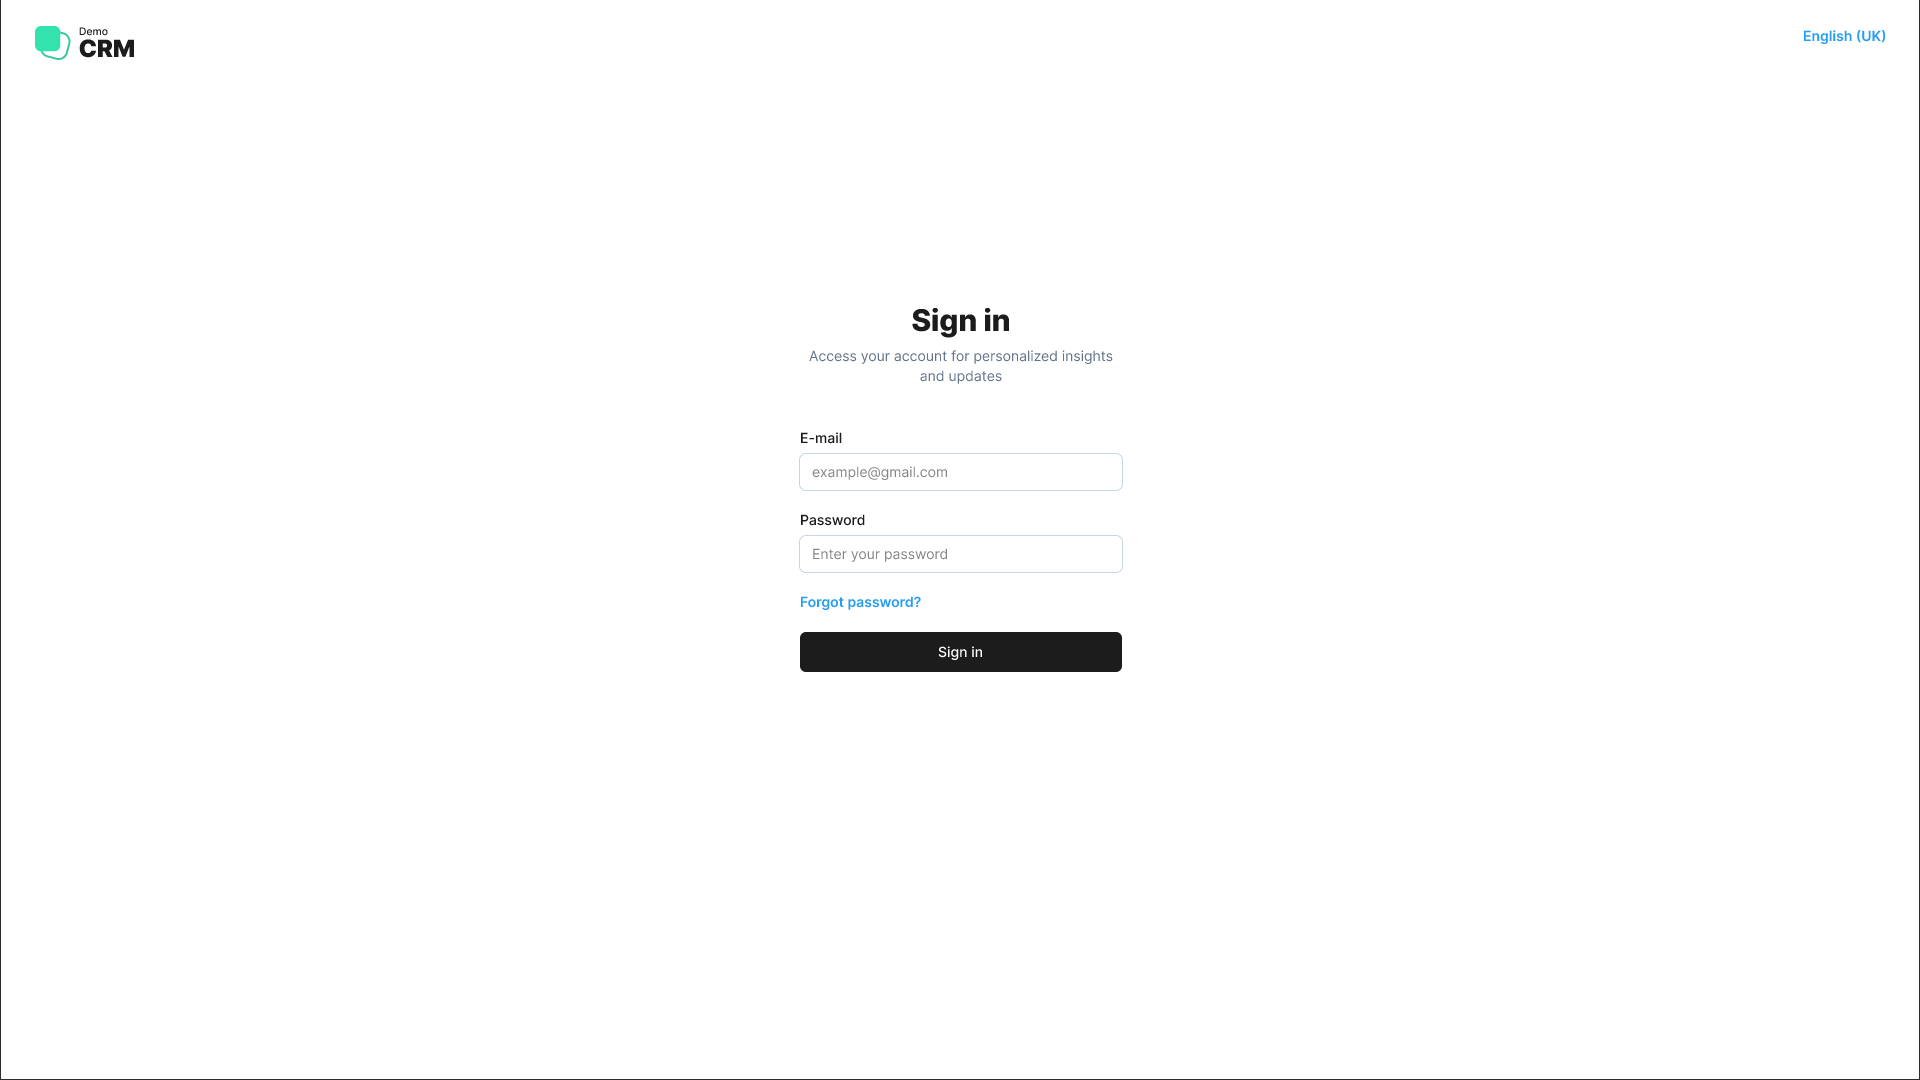
\includegraphics[width=0.9\linewidth]{Images/Sprint1/screenshots/Screenshot 2024-05-26 214007.png}
	\caption{Authentication Interface}
	\label{fig:Authentication Interface}
\end{figure}

\subsection{Email Template Builder}

The email template builder was one of the main features implemented in Sprint 1. I used a drag-and-drop interface for MJML blocks, which allows users to easily design their email templates. The MJML blocks are then rendered into HTML for compatibility with various email clients. This approach provides a balance between ease of use for the user and flexibility in email design.

\begin{figure}[ht]
	\centering
	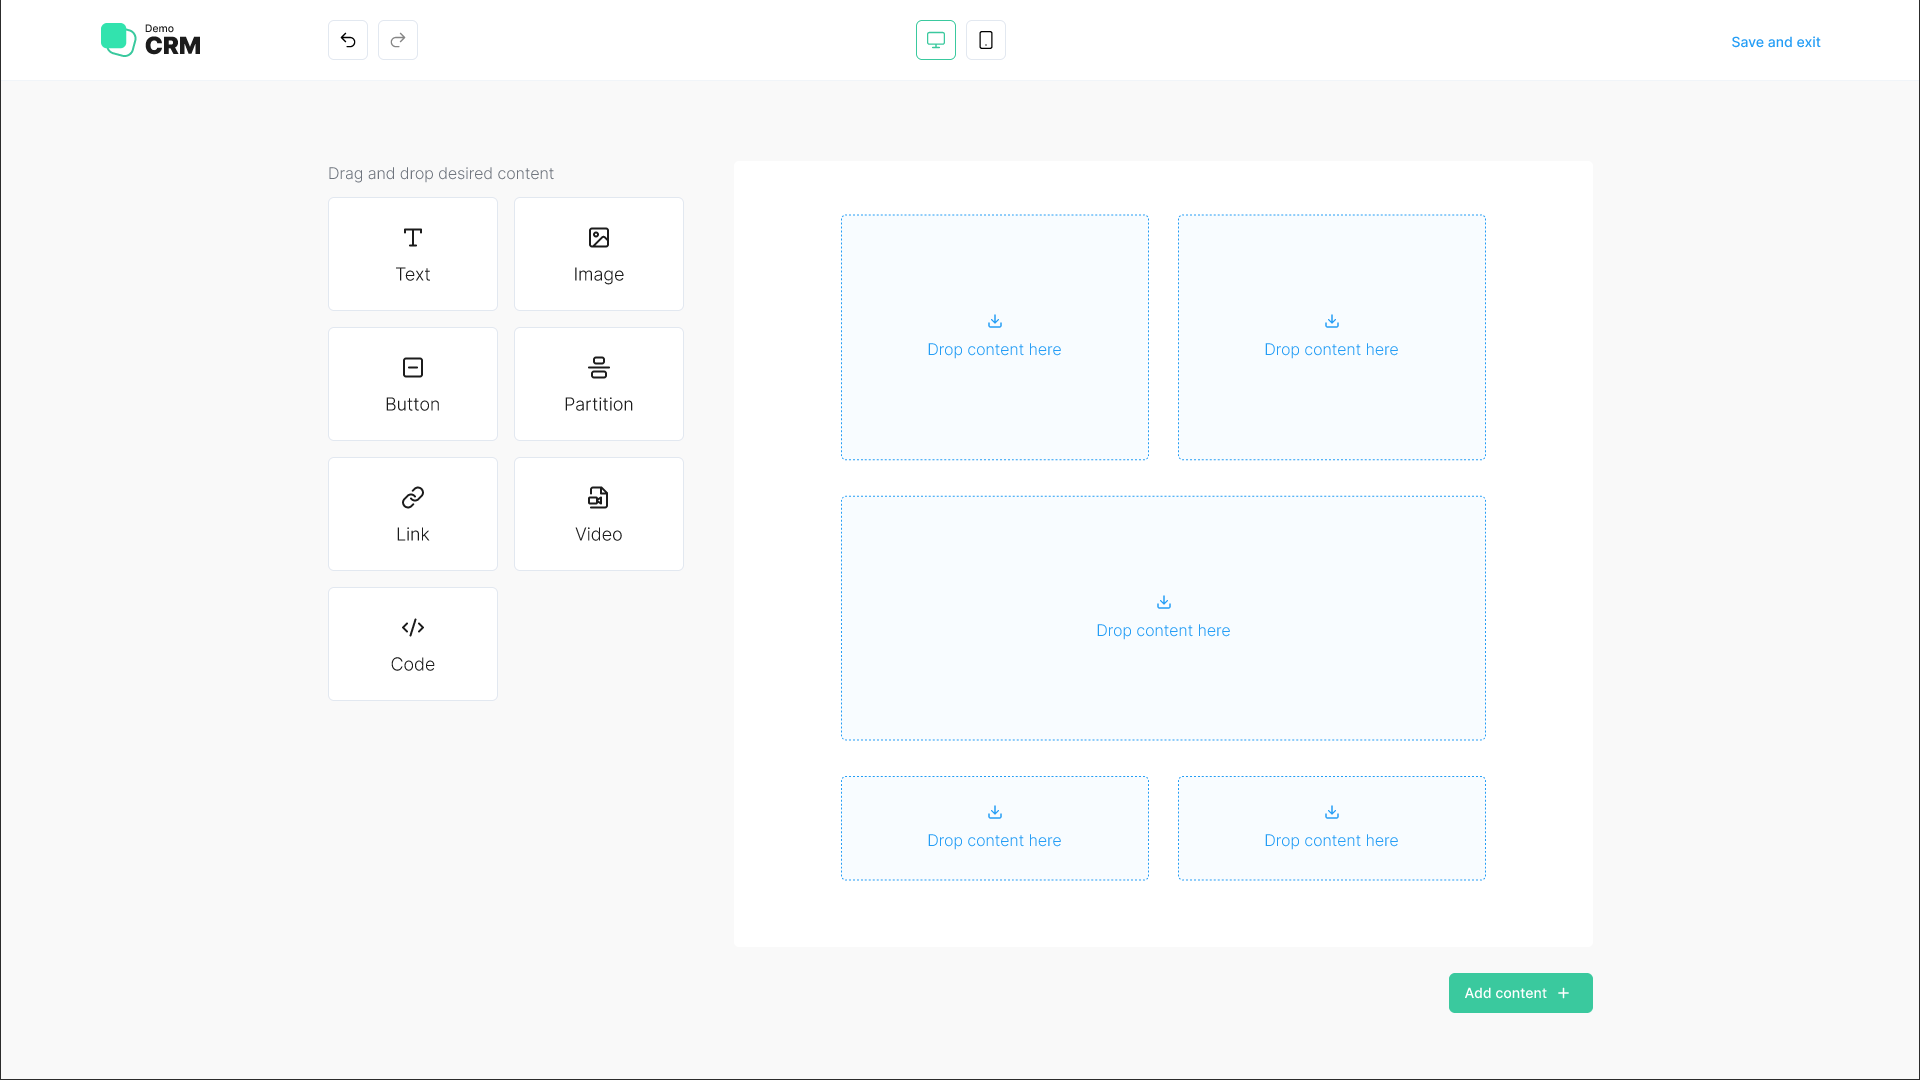
\includegraphics[width=0.9\linewidth]{Images/Sprint1/screenshots/Screenshot 2024-05-26 214054.png}
	\caption{Email Template Builder}
	\label{fig:Email Template Builder}
\end{figure}

\subsection{Email Template Library}

The email template library allows users to save and reuse email templates. Users can create new templates from scratch or save existing templates for future use. This feature is designed to save time and effort for users who frequently send similar emails.

\begin{figure}[ht]
	\centering
	\begin{subfigure}[b]{0.45\linewidth}
		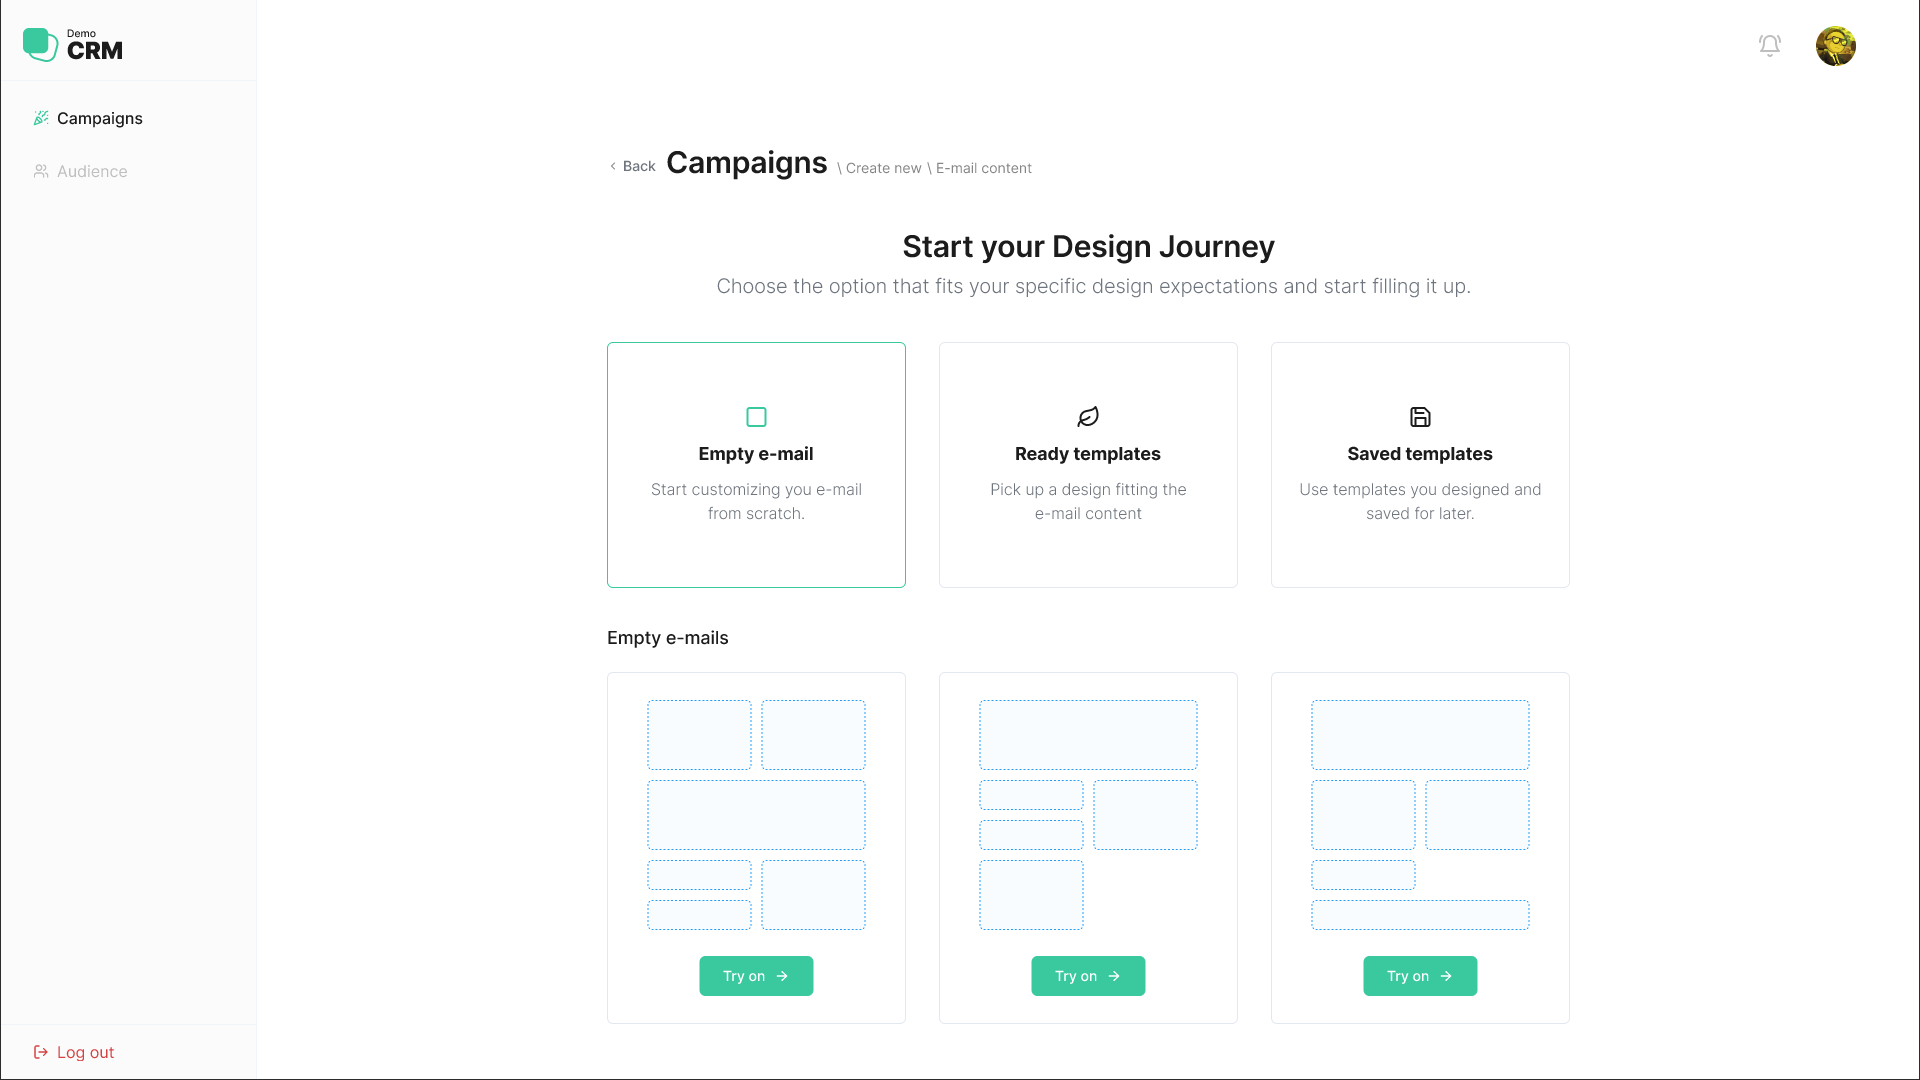
\includegraphics[width=\linewidth]{Images/Sprint1/screenshots/Screenshot 2024-05-26 214037.png}
		\caption{Empty Email Templates Library}
		\label{fig:Empty Email Templates Library}
	\end{subfigure}
	\hfill
	\begin{subfigure}[b]{0.45\linewidth}
		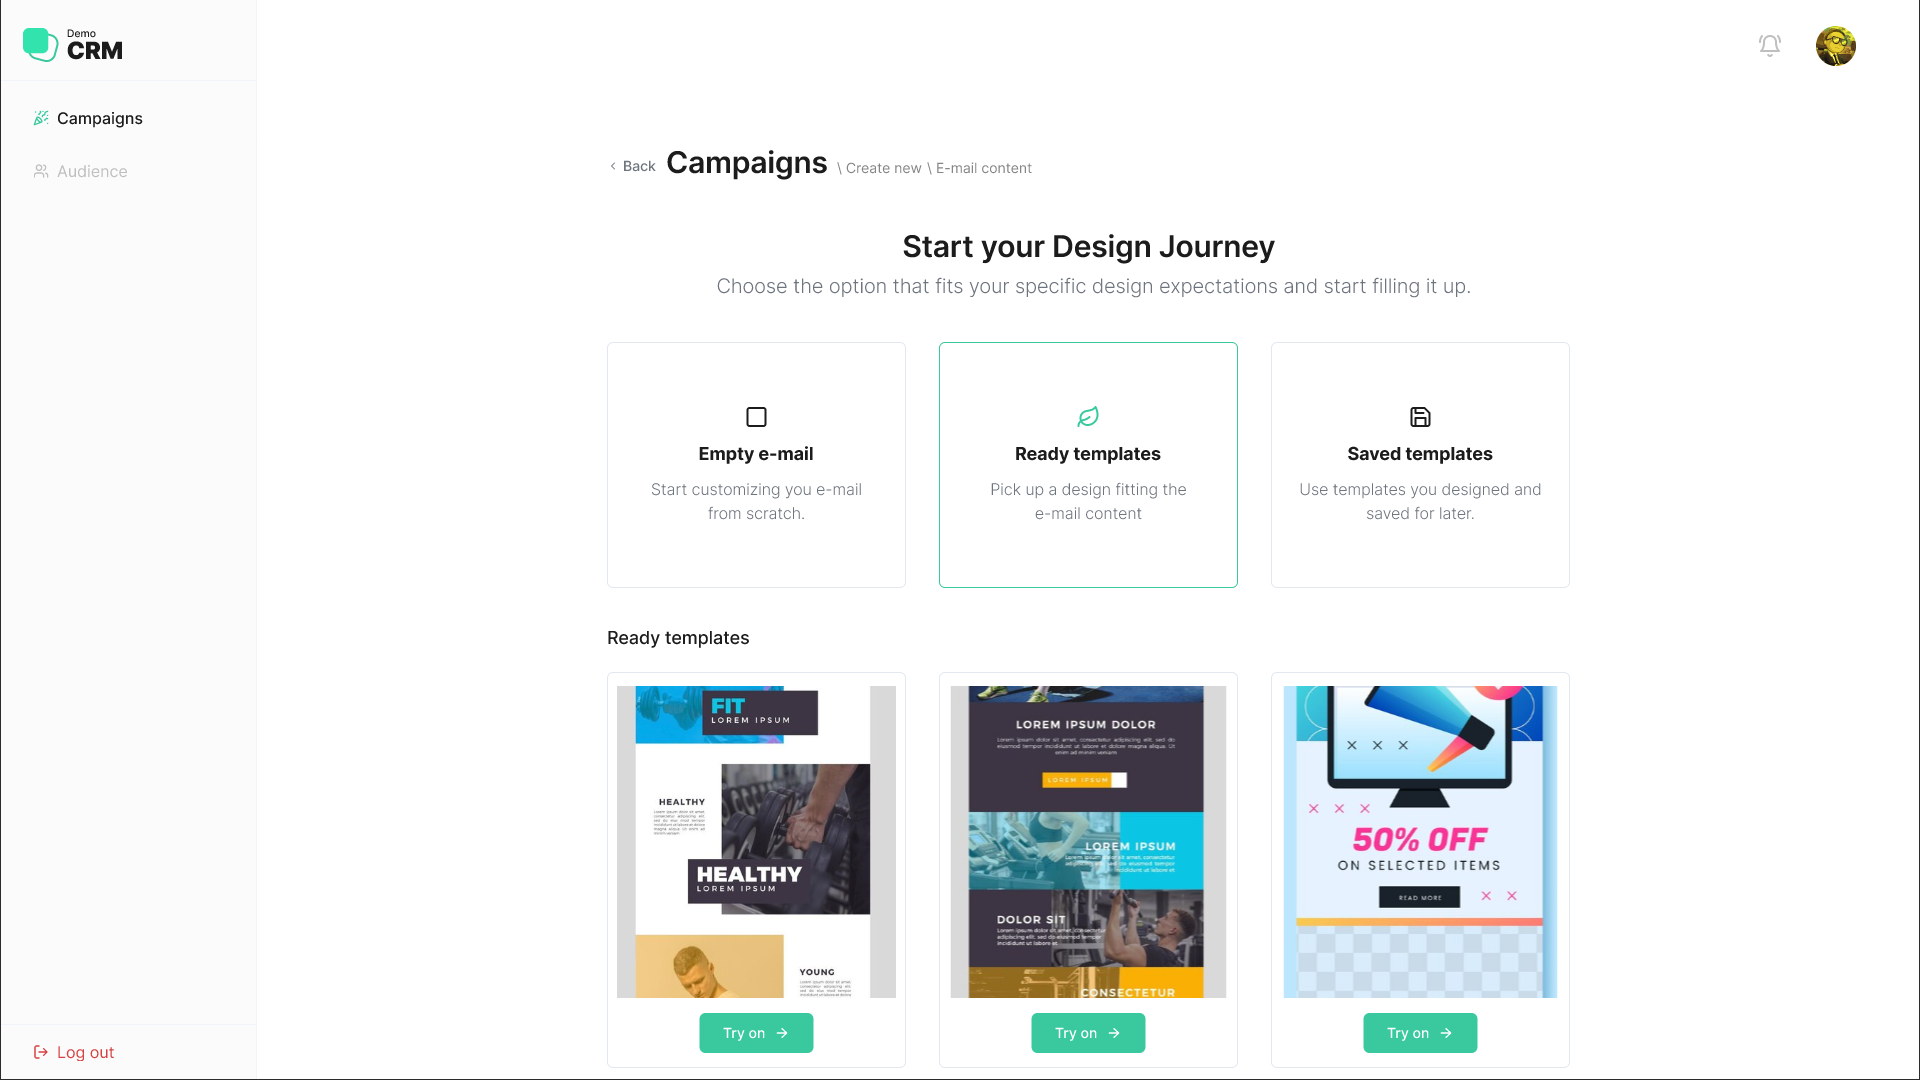
\includegraphics[width=\linewidth]{Images/Sprint1/screenshots/Screenshot 2024-05-26 214047.png}
		\caption{Ready Email Templates library}
		\label{fig:Ready Email Templates library}
	\end{subfigure}
	\caption{Email Template Library}
\end{figure}

\subsection{Campaigns Publishing and Creation}

The functionality for creating and publishing campaigns was also implemented in this sprint. Users can create a campaign, design an email using the template builder, and then publish the campaign to send the email to their audience.

\begin{figure}[ht]
	\centering
	\begin{subfigure}[b]{0.45\linewidth}
		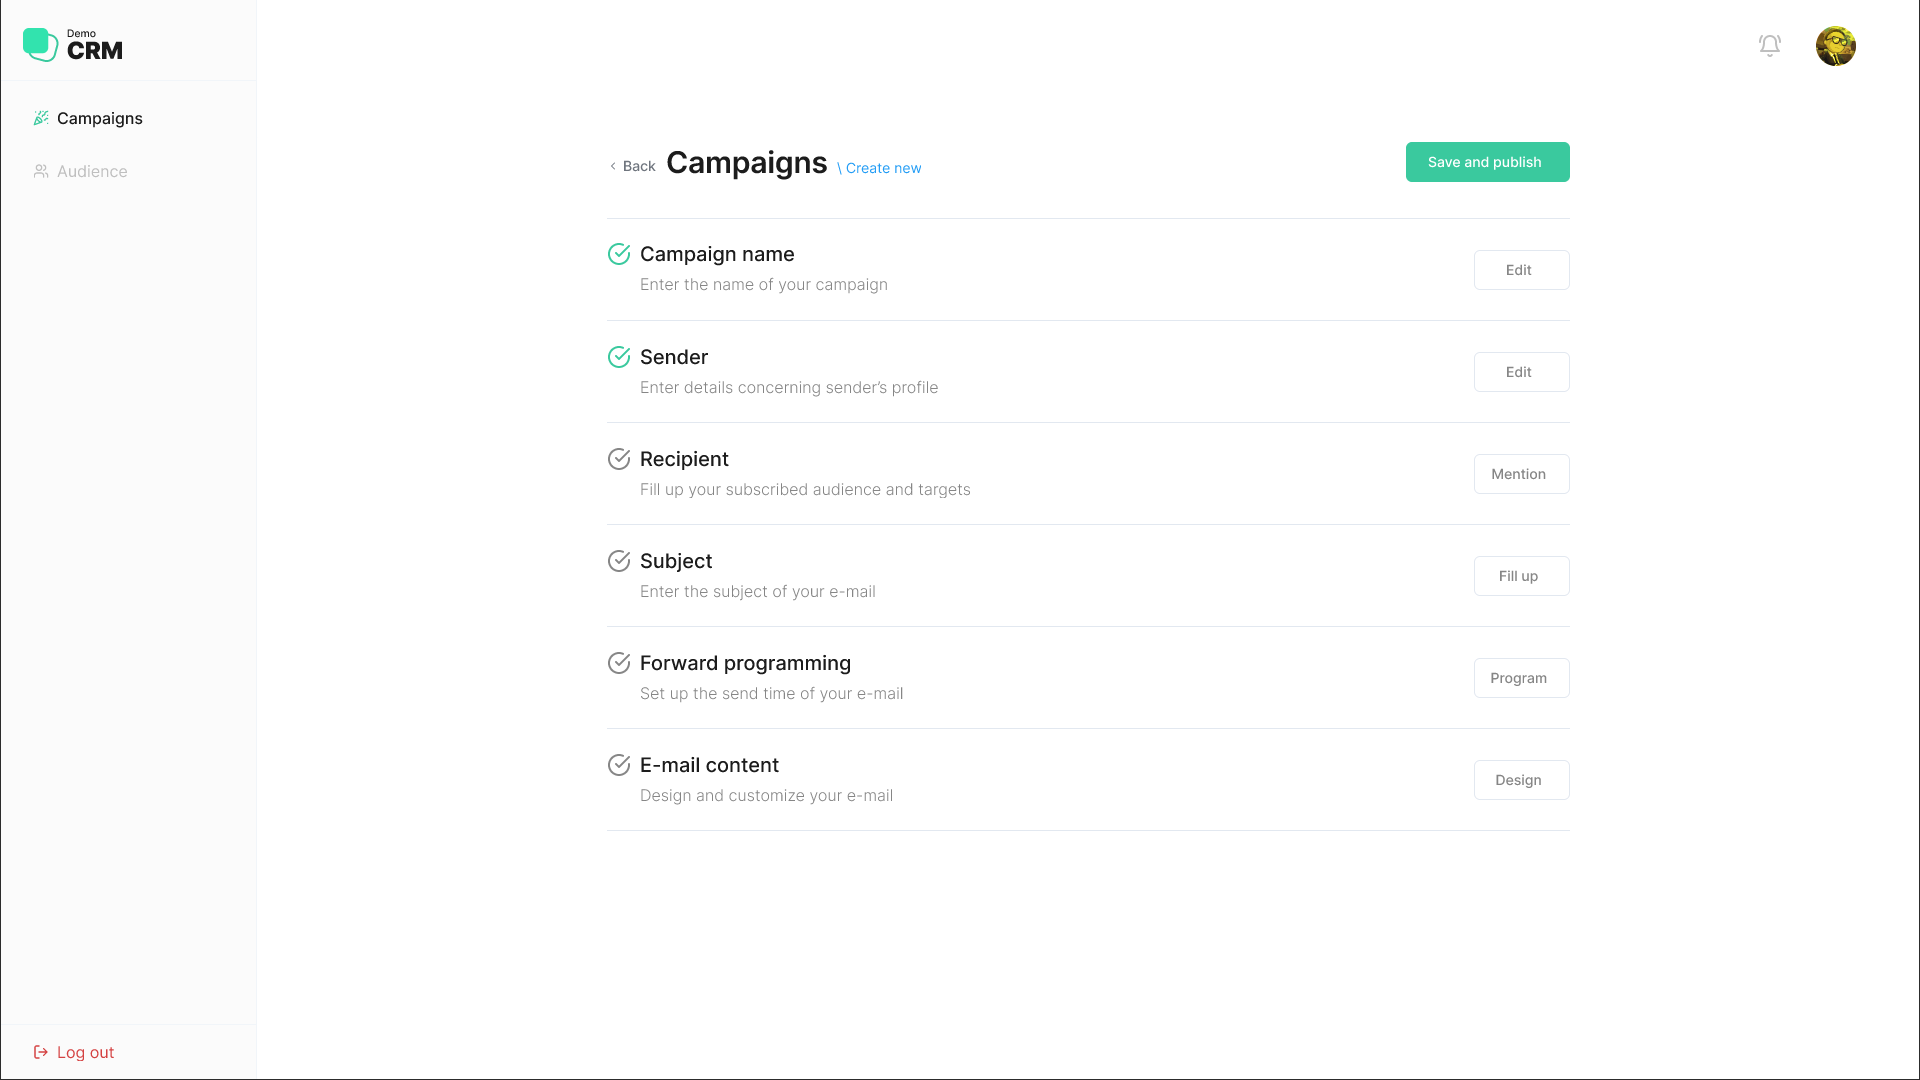
\includegraphics[width=\linewidth]{Images/Sprint1/screenshots/Screenshot 2024-05-26 214028.png}
		\caption{Campaigns Publishing and Creation}
		\label{fig:Campaigns Publishing and Creation}
	\end{subfigure}
	\hfill
	\begin{subfigure}[b]{0.45\linewidth}
		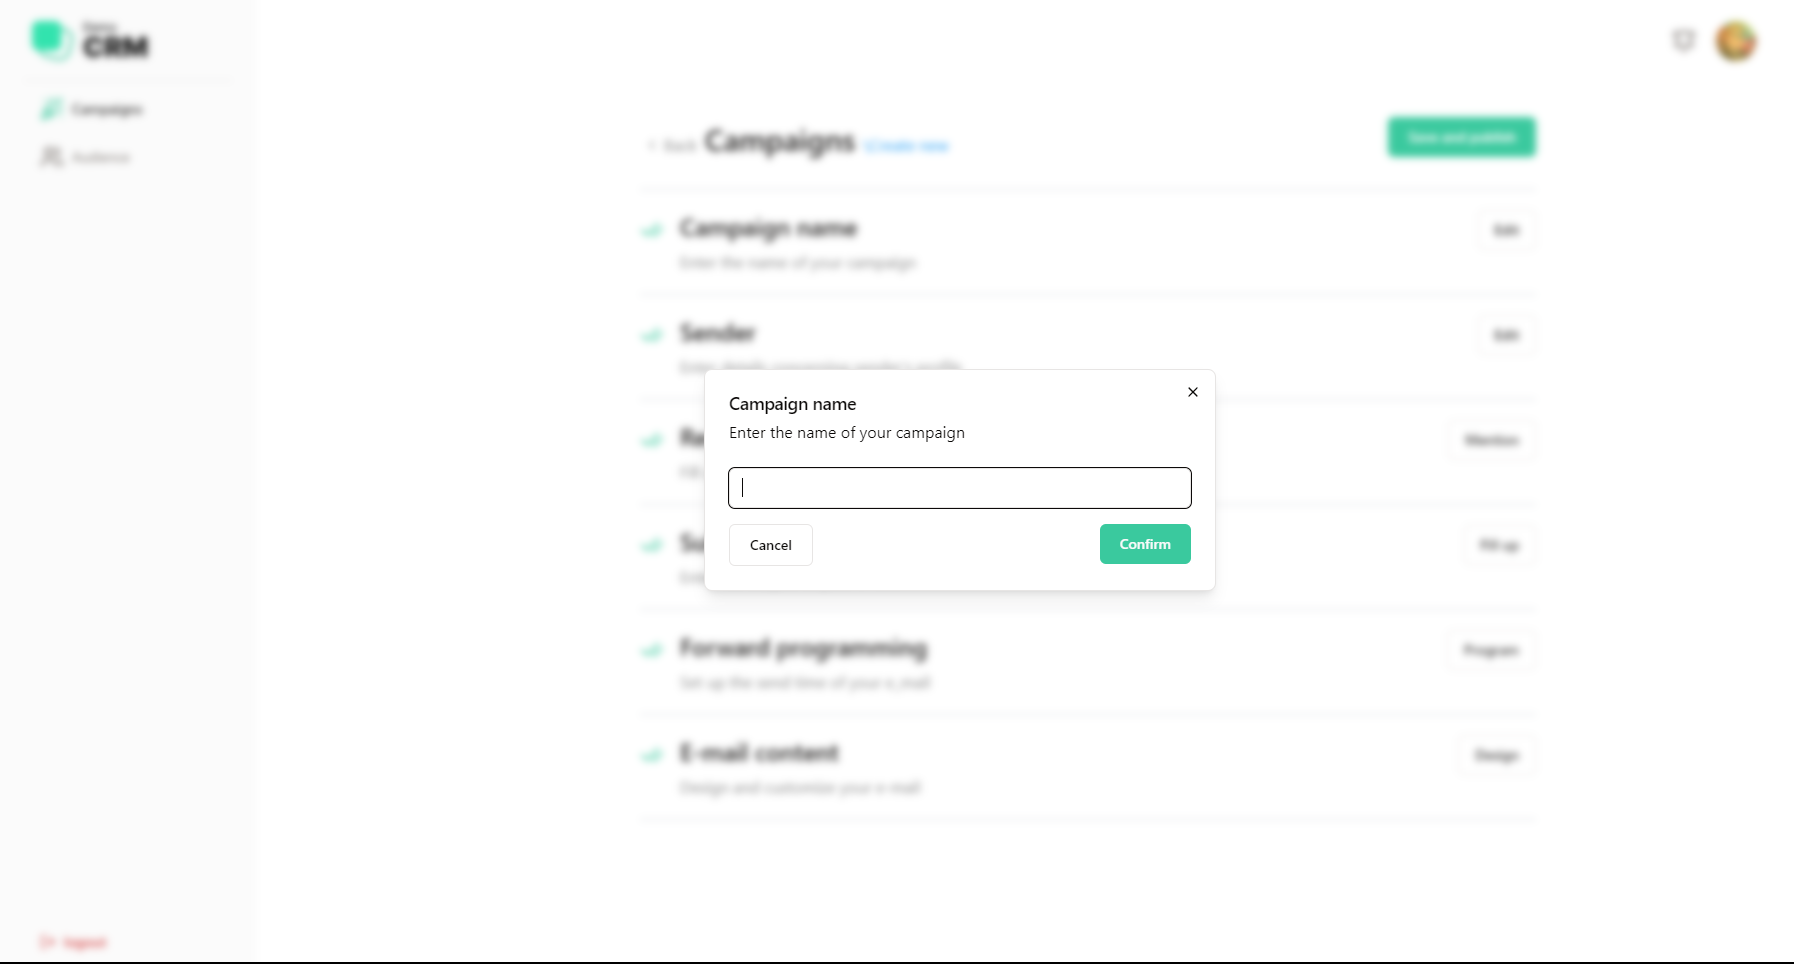
\includegraphics[width=\linewidth]{Images/Sprint1/screenshots/Screenshot 2024-06-03 202916.png}
		\caption{Campaign creation form}
		\label{fig:Campaign creation form}
	\end{subfigure}
	\caption{Campaigns Publishing and Creation}
\end{figure}


\subsection{Campaigns List}

The campaigns listing interface allows users to view and manage their existing campaigns. Users can see a list of all active and past campaigns, along with relevant details such as campaign name, send date, and updating date.
\begin{figure}[ht]
	\centering
	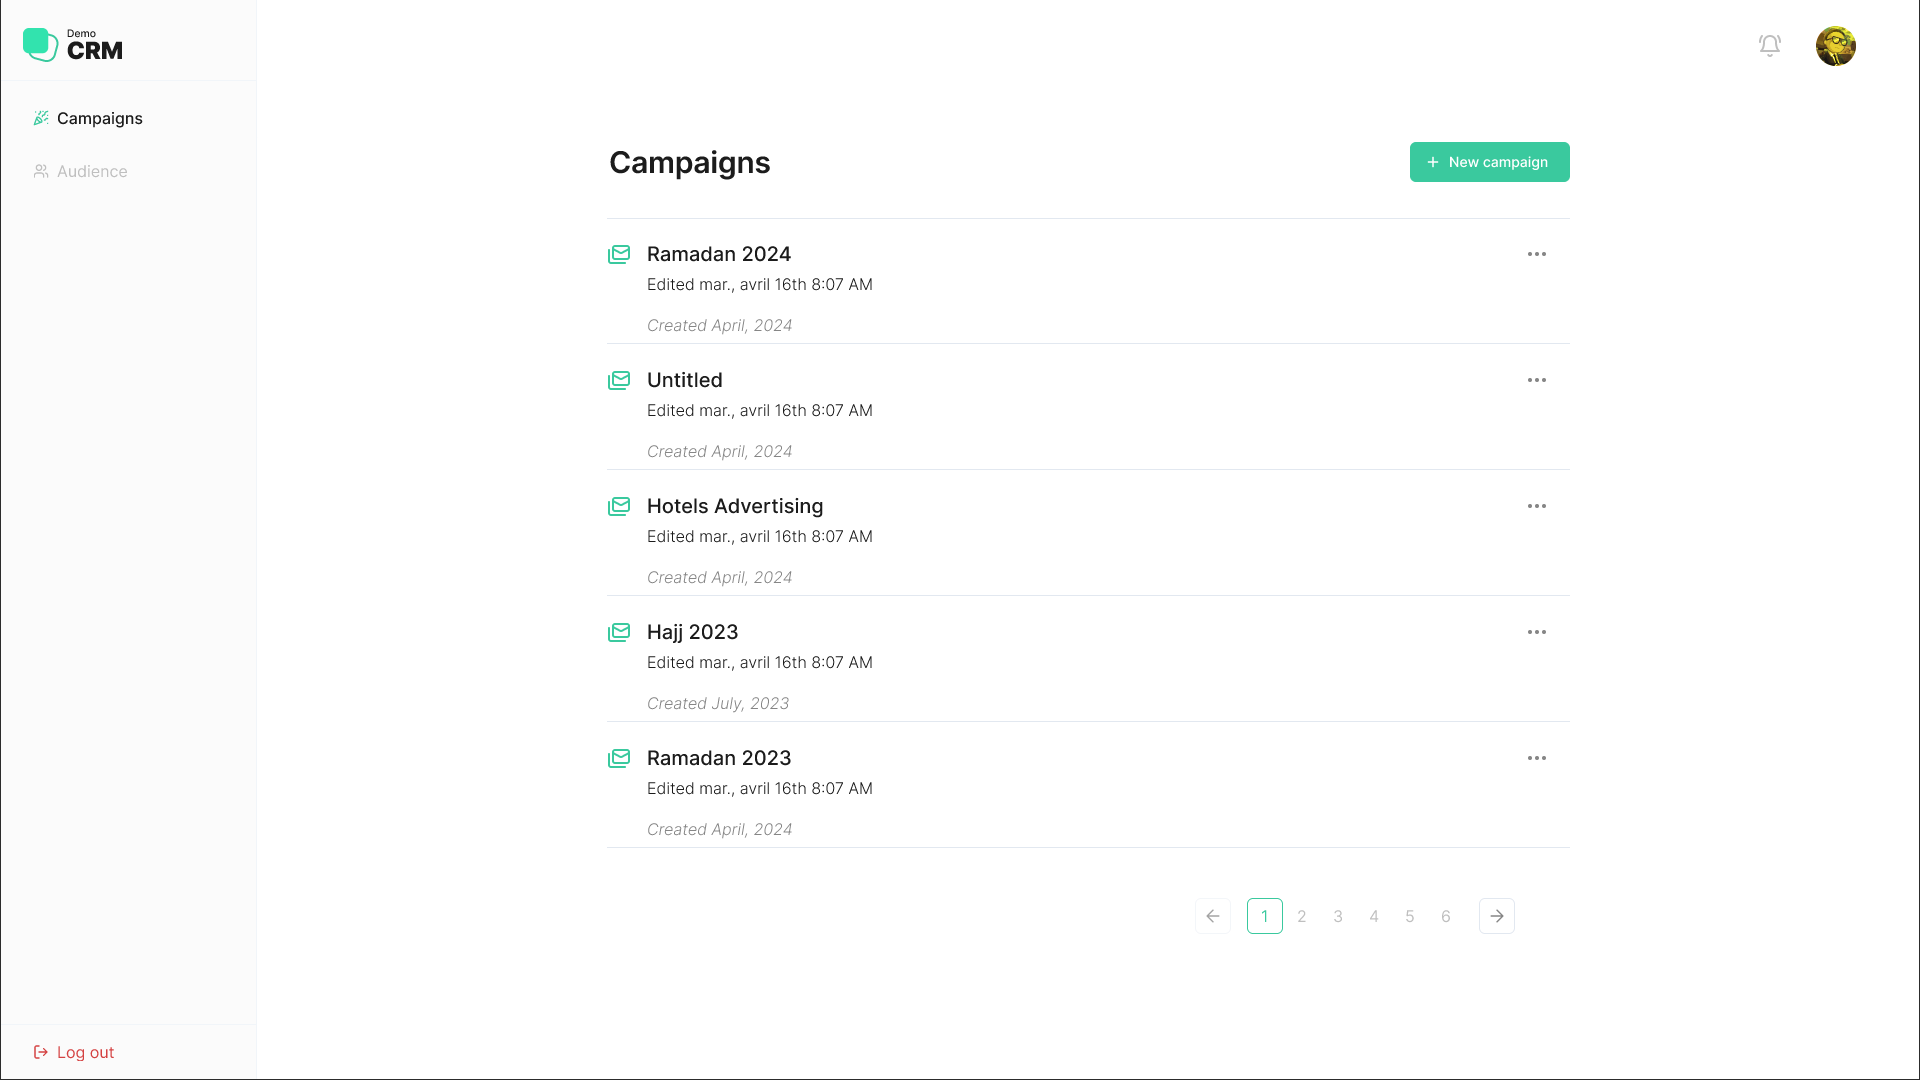
\includegraphics[width=0.9\linewidth]{Images/Sprint1/screenshots/Screenshot 2024-05-26 214015.png}
	\caption{Campaigns List}
	\label{fig:Campaigns List}
\end{figure}
